\subsection{Description du concept}

\paragraph{}
La problématique principale du projet fut de concevoir une architecture logicielle qui reflète le fonctionnement de la console mais qui puisse aussi être modulaire. En effet, les composants de la NES communiquent les uns avec les autres à travers l'espace d'adressage du processeur 6502, la cartouche de jeu y compris. Avec le format cartouche, il est tout à fait possible de moduler le circuit électronique de la cartouche pour augmenter la capacité de stockage du programme ou sauvegarder des parties. Nous constatons alors que l'espace d'adressage varie d'un type de cartouche (ou \emph{mapper} dans le langage technique de la console) à un autre.

\paragraph{}
Nous avons donc développé notre émulateur sur un modèle orienté objet : chaque structure est accompagnée de fonctions constructrice, destructrice et fonctionnelles. Ce modèle nous permet de gagner en modularité : lors d'un chargement de ROM, venir charger l'espace mémoire correspondant au mapper du jeu et ce de manière transparente pour le reste du système. Vous retrouvez sur la figure \ref{fig:struct_app} l'architecture de l'émulateur du point de vue des structures. La structure \emph{NES} contient le modèle de l'émulateur, incluant la structure \emph{CPU}, \emph{PPU} et \emph{Controller}. Toutes ces structures partagent un même pointeur sur la structure \emph{Mapper}, une structure que l'on pourrait décrire comme une classe abstraite en POO puisqu'elle permet au reste du logiciel de s'abstraire du type de mapper utilisé. Comme toutes classes abstraites, il faut définir le comportement de chaque mapper sur la base des fonctions définies. Dans le délai imparti par le projet, nous n'avons pu décrire que le mapper \emph{NROM}, mais il est tout à fait possible d'agrémenter l'émulateur en mapper avec cette architecture logicielle.

\begin{figure}[H]
	\centering
  \subfloat[Structure \emph{App}]{
    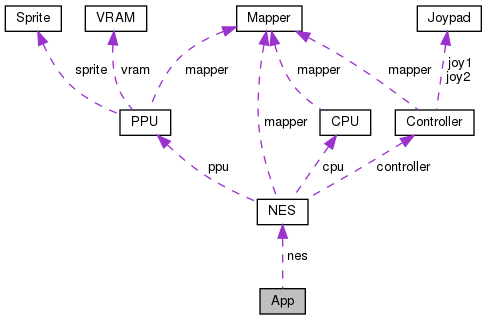
\includegraphics[width=0.45\linewidth]{images/struct_app}
    \label{fig:struct_app}
  }
  \hspace{2cm}
  \subfloat[Structure \emph{MapNROM}]{
    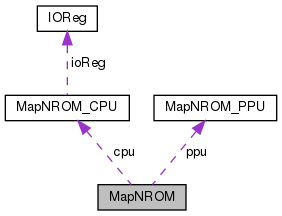
\includegraphics[width=0.25\linewidth]{images/struct_map_nrom}
    \label{fig:struct_map_nrom}
  }
  \caption{Structures de l'émulateur}
  \label{fig:structure}
\end{figure}

\paragraph{}

\subsection{Modèle-vue-contrôleur}

<<<<<<< HEAD
L’émulateur et son environnement graphique est géré par le module App, regroupant le modèle (module NES) avec la vue et le contrôleur (assurés par la SDL). En effet, lors de la modélisation des structures, nous avons pris soin de développer un module NES indépendant de toute technologies d'affichages graphiques et de contrôles, dans le but de pouvoir réutiliser celui-ci dans un contexte différent sans devoir à tout redévelopper. La fonction NES\_NextFrame() est la fonction de plus haut niveau qui permet d'émuler la NES jusqu’à ce qu'une image soit produite. Elle prend en paramètre les touches pressées par l'utilisateur sous forme d'un champ de bits. On récupère par la suite un tableau de pixels correspondant à l'image produite à travers la fonction NES\_Render(). Ce tableau sera exploité par la SDL pour afficher l'image à l'écran. Nous sommes en capacité de forcer l'émulation à la vitesse adéquate en forcant 60 images par secondes, comme le veut le standard NTSC.
=======
L’émulateur et son environnement graphique sont gérés par le module App, regroupant le modèle (module NES) avec la vue et le contrôleur (assurés par la SDL). En effet, lors de la modélisation des structures, nous avons pris soin de développer un module NES indépendant de toutes technologies d'affichages graphiques et de contrôles, dans le but de pouvoir réutiliser celui-ci dans un contexte différent sans devoir à tout redévelopper. La fonction NES\_NextFrame() est la fonction de plus haut niveau qui permet d'émuler la NES jusqu’à ce qu'une image soit produite. Elle prend en paramètre les touches pressées par l'utilisateur sous forme d'un champ de bits. On récupère par la suite un tableau de pixels correspondant à l'image produite à travers la fonction NES\_Render(). Ce tableau sera exploité par la SDL pour afficher l'image à l'écran. Nous sommes en capacité de forcer l'émulation à la vitesse adéquate en forçant 60 images par seconde, comme le veut le standard NTSC.
>>>>>>> a3f6670ec1d427446fb4cd93532384701540a090

\subsection{Moyens de tests}

En plus des tests unitaires, nous avions à disposition des ROMs permettant de tester la conformité de notre émulation. Ces ROMs se trouvent sur \url{nesdev.com}, tout comme les informations sur le fonctionnement de la console sur lequel nous nous sommes basés. Pour tester le bon fonctionnement du processeur 6502, nous exécutons puis comparons les logs que nous avons produits avec celui fourni par un programme spécifique. Pour le test de la PPU, les jeux \emph{Donkey Kong} et \emph{Super Mario Bros.} nous ont permis de tester les différentes spécificités et cas à difficultés.
